\subsection{bpmnr/nr\_\-seed.c File Reference}
\label{nr__seed_8c}\index{bpmnr/nr\_\-seed.c@{bpmnr/nr\_\-seed.c}}


\subsubsection{Detailed Description}


Definition in file {\bf nr\_\-seed.c}.

{\tt \#include $<$bpm/bpm\_\-messages.h$>$}\par
{\tt \#include $<$bpm/bpm\_\-nr.h$>$}\par


Include dependency graph for nr\_\-seed.c:\nopagebreak
\begin{figure}[H]
\begin{center}
\leavevmode
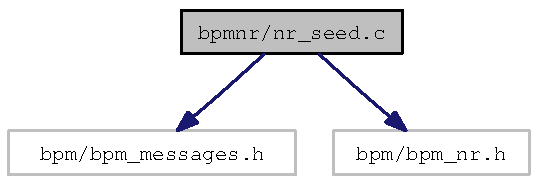
\includegraphics[width=147pt]{nr__seed_8c__incl}
\end{center}
\end{figure}
\subsubsection*{Functions}
\begin{CompactItemize}
\item 
int {\bf nr\_\-seed} (long seed)
\end{CompactItemize}
\subsubsection*{Variables}
\begin{CompactItemize}
\item 
long {\bf bpm\_\-rseed}
\end{CompactItemize}


\subsubsection{Variable Documentation}
\index{nr\_\-seed.c@{nr\_\-seed.c}!bpm\_\-rseed@{bpm\_\-rseed}}
\index{bpm\_\-rseed@{bpm\_\-rseed}!nr_seed.c@{nr\_\-seed.c}}
\paragraph[bpm\_\-rseed]{\setlength{\rightskip}{0pt plus 5cm}long {\bf bpm\_\-rseed}}\hfill\label{nr__seed_8c_c988f9e1a0efc51f61aa8731b011a44b}


the global random seed variable 

Definition at line 9 of file nr\_\-seed.c.

Referenced by nr\_\-rangauss(), nr\_\-ranuniform(), and nr\_\-seed().